\chapter{Control and navigation of the leader drone over 5G network}

\section{Introduction}

In this chapter, we perform a comparative analysis to examine how linear and nonlinear controllers impact quadrotor performance when operated via cellular or 5G networks. This simulation is part of the Ericsson 5G Lab's efforts in autonomous vehicle technology, encompassing both simulation and implementation of UAVs and UGVs navigating over a 5G network. The project is divided into two phases. The first phase focuses on studying the control mechanisms of autonomous vehicles, taking into account delay constraints. The second phase involves developing a practical testbed for evaluating the designed algorithms.

In this project, we consider a scenario where a single UAV is flown over a 5G network, controlled remotely by a user from a station. This section outlines the challenges encountered and presents solution to address these challenges. Regarding the simulation aspect, we choose to run the controller at the Ground Control Station due to the following reasons:

\begin{itemize}
	\item \textit{Integrated control system}: The controller uses information provided by the delay estimator and state estimator. All these parts should be run as an integrated system on the  Ground Control Station to avoid the interconnection delay among the controller, state estimator, and delay estimator.
	\item \textit{Low computation time}: Running complex control systems needs high computation capability that the servers can provide on the  Ground Control Station. 
	\item \textit{Beamforming}: The beamforming technology needs the user's current position to find the most efficient data delivery route. In the studied control framework, the  Ground Control Station provides the drone's position to the base station.
	\item \textit{Path planning}: The controller executes the commands that are provided by a path planning algorithm. The proposed framework reduces the transmission delay between the path planning algorithm and the control system.
\end{itemize}
	
Fig.~\ref{fig3_1:ControlFramework} shows the control framework. The controller sends control commands $U(t)$ to the quadrotor using the cellular networks. The quadrotor receives control commands and sends back position and orientation $S(t)$. The recorded delay history is used for time delay estimation ($\hat{\tau}_B$).

\begin{figure}[H]
	\centering
	\includegraphics[scale=0.5]{Figures/ControlFramework.pdf}
	\caption{Control framework for quadrotor control using cellular networks}
	\label{fig3_1:ControlFramework}
\end{figure}

The state estimator estimates the quadrotors current position and orientation $\hat{S}(t)$ using delay information, control commands, and received data from the quadrotor.

\section{Quadrotor dynamic model}

In this section, the dynamic model of the quadrotor is presented. The quadrotor is a six Degree-of-Freedom (DOF) system controlled by four motors, as shown in Fig.~\ref{fig3_2:QuadrotorModel}. It is an underactuated system that makes the control process a challenging task.

\begin{figure}[H]
	\centerline{\includegraphics{Figures/DroneModel.pdf}}
	\caption{Quadrotor's dynamic model}
	\label{fig3_2:QuadrotorModel}
\end{figure}

An inertial $\left\lbrace O_{I},x,y,z\right\rbrace$ and a body-fixed $\left\lbrace O_{B},x_b,y_b,z_b\right\rbrace$ reference frame are used to define the rotational and transitional motions \cite{Ch4_DM}. According to rigid body dynamics, the rotational motion can be represented as,

\begin{equation}
	\ddot{\phi}=\frac{\left(I_y-I_z\right)}{I_x}\dot{\theta}\dot{\psi}+\frac{l}{I_x}U_2
	\label{QDM1}
\end{equation}

\begin{equation}
	\Ddot{\theta} = \frac{(I_{z} - I_{x})}{I_{y}}\dot{\phi}\dot{\psi} + \frac{l}{I_{y}}U_3
	\label{QDM2}
\end{equation}

\begin{equation}
	\Ddot{\psi} = \frac{(I_{x} - I_{y})}{I_{z}}\dot{\theta}\dot{\phi} + \frac{l}{I_{z}}U_4
	\label{QDM3}
\end{equation}

\noindent where, $\left\lbrace \phi,\theta,\psi\right\rbrace$ are the Euler angles (pitch, roll, and yaw), $I_{x}$, $I_{y}$, and $I_{z}$ are the moment of inertia along $x$, $y$, and $z$ axes, respectively. The $U_{i}$s are the control inputs, and $l$ is the distance between the quadrotor's geometric center and the rotors. 

The transitional motion in the inertial frame is given by,

\begin{equation}
	\Ddot{x} = \left( \cos\phi \sin\theta \cos\psi + \sin\phi \sin\psi \right)\frac{U_1}{m}
	\label{QDM4}
\end{equation}

\begin{equation}
	\Ddot{y} = \left( \cos\phi \sin\theta \sin\psi - \sin\phi \cos\psi \right)\frac{U_1}{m}
	\label{QDM5}
\end{equation}

\begin{equation}
	\Ddot{z} = -g + \left( \cos\phi \cos\theta \right)\frac{U_1}{m}
	\label{QDM6}
\end{equation}

\noindent where, $m$ is the mass, and $g$ is the acceleration due to gravity. The generated force by the motors is considered to be proportional to the square of the angular velocities of the rotors. Therefore, the control inputs can be represented as,

\begin{equation}
	U_{1} = b\left( \omega_1^2 + \omega_2^2 + \omega_3^2 + \omega_4^2 \right)
	\label{QDM7}
\end{equation}

\begin{equation}
	U_{2} = b\left( \omega_4^2 - \omega_2^2 \right)
	\label{QDM8}
\end{equation}

\begin{equation}
	U_{3} = b\left( \omega_3^2 - \omega_1^2 \right)
	\label{QDM9}
\end{equation}

\begin{equation}
	U_{4} = d\left( \omega_2^2 + \omega_4^2 - \omega_1^2 - \omega_3^2 \right)
	\label{QDM10}
\end{equation}

\noindent where, $\omega_{i}$ is the angular velocity of the $i$th rotor, and $b$ and $d$ are constants.

\section{Linear PD Controller}

The PID controller is a widely used linear controller and is defined as,

\begin{equation}
	u(t)=K_pe(t)+K_i\int_{0}^{t}{e(\tau)d\tau}+K_d\frac{de(t)}{dt}
	\label{PD0}
\end{equation}

\noindent where, $e(t)$ is the error between the desired state and the current state, and $K_p$, $K_i$, and $K_d$ are PID gains. In this chapter, a PD controller is designed to control the rotational and transitional motions. The controller is designed based on the linearized model of the quadrotor.

To simplify the linearization of the system, we assume that the yaw angle is held constant at zero, and as such, the motion along the $x$-axis is controlled only by the pitch angle $\theta$, and the motion along the $y$-axis is controlled only by the  roll angle $\phi$. We linearized the dynamics for our PD controller design by assuming that the roll and pitch angles are small, which is a reasonable assumption since quadrotors rarely rotate more than 30 degrees during flight. Also, the angular accelerations of roll and pitch are equal to the torque about the appropriate axis, as such, we write the linear dynamics as $ \ddot{\phi} = T_x/Ixx$ and $\ddot{\theta} = T_y/Iyy$, where $T_x$ and $T_y$ are the torques about the $x$ and $y$-axis.

There are two control loops: inner and outer loop. The outer loop controls the desired pitch and roll angles. Since the motions along $x$ and $y$ axes depend on the rotation along $\phi$ and $\theta$, the outer loop uses the current position in $x$ and $y$ and desired positions to calculate the desired rotations along $x$ and $y$ axes as follows \cite{Ch4_PD1},
\begin{equation}
	\theta_{d} = K_{p}\left( x - x_{d} \right) + K_{d}\left( \dot{x} - \dot{x}_{d} \right)
	\label{PD1}
\end{equation}

\begin{equation}
	\phi_{d} = K_{p}\left( y - y_{d} \right) + K_{d}\left( \dot{y} - \dot{y}_{d} \right)
	\label{PD2}
\end{equation}

\noindent where, $\phi_{d}$ and $\theta_{d}$ are desired pitch and roll angles, and $x_{d}$ and $y_{d}$ are desired positions on $x$ and $y$ directions. The $K_{p}$ and $K_{d}$ control the pitch and roll angles. The inner loop controls the quadrotor's rotation along the $x$ and $y$ axes.

According to the PD control law, the control signals can be represented as \cite{Ch4_PD2},

\begin{equation}
	U_{1} = mg + K_{zp}\left( z_{d} - z  \right) + K_{zd}\left( \dot{z}_{d} - \dot{z} \right)
	\label{PD3}
\end{equation}

\begin{equation}
	U_{2} = K_{lp}\left( \phi_{d} - \phi \right) + K_{ld}\left( \dot{\phi}_{d} - \dot{\phi} \right)
	\label{PD4}
\end{equation}

\begin{equation}
	U_{3} = K_{mp}\left( \theta_{d} - \theta \right) + K_{md}\left( \dot{\theta}_{d} - \dot{\theta} \right)
	\label{PD5}
\end{equation}

\begin{equation}
	U_{4} = K_{np}\left( \psi_{d} - \psi \right) + K_{nd}\left( \dot{\psi}_{d} - \dot{\psi} \right)
	\label{PD6}
\end{equation}

\noindent where, $K_{zp}$, $K_{zd}$, $K_{lp}$, $K_{ld}$, $K_{mp}$, $K_{md}$, $K_{np}$, and $K_{nd}$ are PD gains for the inner loop. The $z_d$ is the desired position along the $z$-axis, and $\psi_{d}$ is the desired yaw angle. 

The linearized PD controller can be designed based on the second-order dynamic model, where the bandwidth and damping ratio of the controller are adjustable. Therefore, gains can be calculated based on the inner and outer loop bandwidth.

\section{Backstepping Controller}

In this section, a nonlinear backstepping control law is designed to be compared with the linear PD controller. As mentioned before, the backstepping controller breaks the control law into several subsystems \cite{Ch4_BS1}. There are three subsystems consisting of the altitude ($z$), heading ($\psi$), and horizontal subsystems. The general Lyapunov function for every subsystem based on error variables is defined as \cite{Ch4_sharma2021control},

\begin{equation}
	V_i=\frac{1}{2}\eta_i^2
	\label{BS3}
\end{equation}

\noindent where, $\eta_i$ is the error variable for the $i$th subsystem.

We define error variables for the $z$ subsystem as $\eta_{1}=z-z_d$, $\eta_{2}=\dot{z}-c_1\eta_1-{\dot{z}}_d$. Then, the control law for altitude control becomes:
	
\begin{equation}
	U_1=\frac{m}{\cos{\phi}\cos{\theta}}\left(g-\eta_1-c_2\eta_2-c_1\dot{z}+c_1{\dot{z}}_d+{\ddot{z}}_d\right)
	\label{BSU1}
\end{equation}

\noindent where, $c_1$ and $c_2$ are constant values that control how fast the quadrotor responds to the input commands in the $z$-direction.

For the $\phi$ subsystem, the error variables are $\eta_{9}=\phi-\phi_d$ and $\eta_{10}=\dot{\phi}-c_9\eta_9-{\dot{\phi}}_d$. Therefore, the control law is given by:

\begin{equation}
	U_2=\frac{I_x}{l}\left(-\alpha\dot{\theta} \dot{\psi}-c_9\dot{\phi}+c_9{\dot{\phi}}_d-\eta_9-c_{10}\eta_{10}+{\ddot{\phi}}_d\right)
	\label{BSU2}
\end{equation}

\noindent where, $\alpha=\frac{I_y-I_z}{I_x}$, and $c_9$ and $c_{10}$ are the constant values that control the response time of the $\phi$ subsystem \cite{Ch4_BS2}.

For the $\theta$ subsystem, the error variables are $\eta_{11}=\theta-\theta_d$ and $\eta_{12}=\dot{\theta}-c_{11}\eta_{11}-{\dot{\theta}}_d$. Then, the control law for the $\theta$ subsystem becomes,

\begin{equation}
	U_3=\frac{I_y}{l}\left(-\beta\dot{\phi} \dot{\psi}-c_{11}\dot{\theta}+c_{11}{\dot{\theta}}_d-\eta_{11}-c_{12}\eta_{12}+{\ddot{\theta}}_d\right)
	\label{BSU3}
\end{equation}

In the above equation, the $\beta=\frac{I_z-I_x}{I_y}$, and $c_{11}$ and $c_{12}$ are the constant values that control the response time of the $\theta$ subsystem.

The error variables for the $\psi$ subsystem are $\eta_{3}=\psi-\psi_d$ and $\eta_{4}=\dot{\psi}-c_{3}\eta_{3}-{\dot{\psi}}_d$. The control law is given by:

\begin{equation}
	U_4=I_z\left(-\gamma\dot{\phi} \dot{\theta}-c_3\dot{\psi}+c_3{\dot{\psi}}_d-\eta_3-c_4\eta_4+{\ddot{\psi}}_d\right)
	\label{BSU4}
\end{equation}

\noindent where, $\gamma=\frac{I_x-Iy}{I_z}$, and $c_{3}$ and $c_{4}$ control the response time of the $\psi$ subsystem. 

Since the dynamic model is underactuated and the $U_1$ is incorporated in $x$ and $y$ subsystems, the virtual control signals in $x$ and $y$ directions can be calculated based on the mentioned Lyapunov function as follows,

\begin{equation}
	\label{BS5}
	u_y=\frac{m}{U_1}\left(-c_5\dot{y}+{c_5\dot{y}}_d+{\ddot{y}}_d-c_6\eta_6-\eta_5\right)
\end{equation}

\begin{equation}
	\label{BS6}
	u_x=\frac{m}{U_1}\left(-c_7\dot{x}+c_7{\dot{x}}_d+{\ddot{x}}_d-c_8\eta_8-\eta_7\right)
\end{equation}

\noindent where, $c_5$ to $c_7$ are constant coefficients, $\eta_5=y-y_d$, $\eta_6=\dot{y}+c_5\eta_5-{\dot{y}}_d$, $\eta_7=x-x_d$, and $\eta_8=\dot{x}+c_7\eta_7-{\dot{x}}_d$ are error values for position and velocity.

The desired roll and pitch angles considering yaw angle are $\phi_d={sin}^{-1}[v(2)]$ and $\theta_d={sin}^{-1}\left[\frac{v(1)}{cos{\phi_d}}\right]$ where,


\begin{equation}
	v=\left[\begin{matrix}cos{\psi}&sin{\psi}\\sin{\psi}&-cos{\psi}\\\end{matrix}\right]^{-1}\left[\begin{matrix}u_x&u_y\\\end{matrix}\right]^T
	\label{BS9}
\end{equation}

The $v$ is designed to find the desired orientation along the $x$ and $y$ axes that make the quadrotor follow the desired position, velocity, and acceleration in the horizontal subsystem.

\section{State Estimator} 

Practical networked control systems with feedback loops are prone to face anomalies due to communication imperfections such as time delay. The feedback loop provides information about the plant's current states, and the controller calculates the new commands based on the received information.

When the system experiences a time delay, the controller may become unstable. In order to design a suitable control system, one should use a state estimator that estimates the current states based on the received data from the plant. In this section, the state estimator is given as follows,

\begin{equation}
	\dot{\hat{\phi}}={\bar{q}}_\phi-k_1\left(\hat{\phi}(t-\hat{\tau}_B)-\phi(t-\tau_B)\right)
	\label{SP1}
\end{equation}

\begin{equation}
	{\dot{\bar{q}}}_\phi=\left(\frac{I_y-I_z}{I_x}\right){\bar{q}}_\theta{\bar{q}}_\psi+\frac{U_2\left(t\right)}{I_x}-k_2\left({\bar{q}}_\phi(t-\hat{\tau}_B)-q_\phi(t-\tau_B)\right)
	\label{SP2}
\end{equation}

\begin{equation}
	\dot{\hat{\theta}}={\bar{q}}_\theta-k_3\left(\hat{\theta}(t-\hat{\tau}_B)-\theta(t-\tau_B)\right)
	\label{SP3}
\end{equation}

\begin{equation}
	{\dot{\bar{q}}}_\theta=\left(\frac{I_z-I_x}{I_y}\right){\bar{q}}_\phi{\bar{q}}_\psi+\frac{U_3\left(t\right)}{I_y}-k_4\left({\bar{q}}_\theta(t-\hat{\tau}_B)-q_\theta(t-\tau_B)\right)
	\label{SP4}
\end{equation}

\begin{equation}
	\dot{\hat{\psi}}={\bar{q}}_\psi-k_5\left(\hat{\psi}(t-\hat{\tau}_B)-\psi(t-\tau_B)\right)
	\label{SP5}
\end{equation}

\begin{equation}
	{\dot{\bar{q}}}_\psi=\left(\frac{I_x-I_y}{I_z}\right){\bar{q}}_\phi{\bar{q}}_\theta+\frac{U_4\left(t\right)}{I_z}-k_6\left({\bar{q}}_\psi(t-\hat{\tau}_B)-q_\psi(t-\tau_B)\right)
	\label{SP6}
\end{equation}


\begin{equation}
	\dot{\hat{x}}={\bar{q}}_x-k_7\left(\hat{x}\left(t-\hat{\tau}_B\right)-x\left(t-\tau_B\right)\right)
	\label{SP7}
\end{equation}

\begin{equation}
	\label{SP8}
	{\dot{\bar{q}}}_x\ =\ \left(\cos{\hat{\phi}}\sin{\hat{\theta}}\cos{\hat{\psi}}+\sin{\hat{\phi}}\sin{\hat{\psi}}\right)\frac{U_1(t)}{m}-k_8\left({\bar{q}}_x\left(t-\hat{\tau}_B\right)-q_x\left(t-\tau_B\right)\right)
\end{equation}

\begin{equation}
	\dot{\hat{y}}={\bar{q}}_y-k_9\left(\hat{y}\left(t-\hat{\tau}_B\right)-y\left(t-\tau_B\right)\right)
	\label{SP9}
\end{equation}

\begin{equation}
	\label{SP10}
	{\dot{\bar{q}}}_y\ =\ \left(cos{\hat{\phi}}sin{\hat{\theta}}sin{\hat{\psi}}-sin{\hat{\phi}}cos{\hat{\psi}}\right)\frac{U_1\left(t\right)}{m}-k_{10}\left({\bar{q}}_y\left(t-\hat{\tau}_B\right)-q_y\left(t-\tau_B\right)\right)
\end{equation}

\begin{equation}
	\dot{\hat{z}}={\bar{q}}_z-k_{11}\left(\hat{z}\left(t-\hat{\tau}_B\right)-z\left(t-\tau_B\right)\right)
	\label{SP11}
\end{equation}

\begin{equation}
	{\dot{\bar{q}}}_z\ =-g+\ \left(cos\hat{\phi}\ cos{\hat{\theta}}\right)\frac{U_1\left(t\right)}{m}-k_{12}\left({\bar{q}}_z\left(t-\hat{\tau}_B\right)-q_z\left(t-\tau_B\right)\right)
	\label{SP12}
\end{equation}

According to \eqref{SP1} to \eqref{SP12}, the state estimation is based on the quadrotor's dynamic model and the control signal. Therefore, we need to run the controller on the GCS to have access to control signals for state estimation. As mentioned before, the state estimation results are necessary information for beamforming. The Due to space restrictions, details are left to the reader \cite{Ch4_sharma2021control}. In \eqref{SP1} to \eqref{SP12}, the $\tau_B$ and $\hat{\tau}_B$ are the true and estimated backward delays (the backward and forward delays are assumed to be equal). The $k_i$s are the estimator gains, and $\hat{\phi}$, $\hat{\theta}$, $\hat{\psi}$, $\hat{x}$, $\hat{y}$, and $\hat{z}$ are the estimated orientations and positions.

\section{Delay Estimator}

Network load, node competition, and congestion affect the communication quality. Therefore, considering the network delay as a constant parameter is not a proper assumption. Whenever a packet is sent over the network, the network state changes. Since the delay distribution follows the Markov model \cite{Ch4_ge2013modeling}, Markov-based models are suitable for delay estimation.

In this chapter, the delay is assumed to be a discrete-time, discrete-space stochastic process. In order to simulate the network delays during simulation, a fixed predefined transition matrix can be used as follows,

\begin{equation}
	p_{ij}(n)=P(\tau_{n+1}=j|\tau_n=i)
	\label{DE2}
\end{equation}

\noindent where, $\tau_n$ and $\tau_{n+1}$ are current and next time delays, respectively, and the $i$ and $j$ are indices corresponding with the time delays. The delays estimator algorithm aims to find the true transition probabilities. 

\begin{algorithm}
	\caption{Time delay estimation using Markov model}
	\label{Algorithm3.1}
	\begin{algorithmic}[1]
	\State {\textbf{input} $D_{1\times \lambda}$,  delay values}
	\State {\textbf{input} $M_{\lambda\times \lambda}$, auxiliary matrix}
	\State {\textbf{input} $\hat{p}_{\lambda\times \lambda}$, estimated probability matrix}
	\For{$n$ = $1$ to $simulation\hspace{4pt} time$}
	\State \textbf{read} $\tau(n-1)$
	\State $i \gets$ index of $\tau(n-1)$ in $D$
	\State $j \gets$ index of $\tau(n-2)$ in $D$
	\State $M[j,i] \gets M[j,i] + 1$
	\For{$r = 1$ to $\lambda$}
	\State $\hat{p}[r,1:\lambda] \gets $ Normalize $r^{th}$ row of the $M$
	\EndFor
	\State $ind$  $\gets$ find the index of max($\hat{p}[i,1:\lambda]$)
	\State $\hat{\tau}[n] \gets D[1,ind]$
	\State $DEE(n-1) \gets \sqrt{\frac{\sum_{i=0}^{n-1}\left(\tau(n-1)-\hat{\tau}(n-1)\right)^2}{n-1}}$
	\EndFor
	\end{algorithmic}
\end{algorithm}


The delays are generated based on the fixed predefined transition matrix $p$. Delay values are assumed to be known ($D={\tau_1, \tau_2, ... , \tau_{\lambda}}$), but we do not know which one will happen in the current time step. Therefore, the challenge is to find the transition probabilities matrix $p$. The delay estimator gets the previous delay $\tau(n-1)$ as the initial value and calculates the transition probabilities matrix using the observed delays' history. Finally, the Delay Estimation Error (DEE) is calculated based on the delay history. 

\section{Results}

The performance of the controllers was evaluated using a numerical simulation. The simulation was done in MATLAB R2021 and the total simulation time was 10 seconds with 0.001 second sampling time. The initial condition for orientation, angular velocities, position, and velocities were taken to be $\mathbf{0}_{12\times1}$. The desired positions in the $x$, $y$, and $z$ directions were 10, 20, and 30 $m$.

The PD controller was designed using the linearized model of quadrotor dynamics. The gains were calculated using the second-order system model, and the bandwidth for inner and outer loops were 70 rad/s and 5 rad/s, respectively. High bandwidths for controllers can be used because of the small delay values in the 5G network. The $c_{i}$s in the backstepping controller were tuned so that the response time of the controllers are approximately equivalent. The control gains are shown in Table \ref{Table3.1}. 


\begin{table}
	\caption{Gains used in PD and backstepping controllers}
	\begin{center}
		\begin{tabular}{|lllll|}
			\hline
			& \multicolumn{1}{c}{\multirow{2}{*}{\textbf{Coefficient}}} & \multicolumn{1}{c}{\multirow{2}{*}{\textbf{Value}}} & \multirow{2}{*}{\textbf{Coefficient}} & \multirow{2}{*}{\textbf{Value}} \\
			& \multicolumn{1}{c}{}                                      & \multicolumn{1}{c}{}                                &                                       &                                 \\ \hline
			\multicolumn{1}{|c|}{\multirow{5}{*}{\textbf{PD}}}           & $K_{p}$                                                   & 2.5                                                 & $K_{d}$                               & 1                               \\
			\multicolumn{1}{|c|}{}                                       & $K_{lp}$                                                  & 20.09                                               & $K_{ld}$                              & 0.574                            \\
			\multicolumn{1}{|c|}{}                                       & $K_{mp}$                                                  & 20.09                                               & $K_{md}$                              & 0.574                            \\
			\multicolumn{1}{|c|}{}                                       & $K_{np}$                                                  & 43.12                                                  & $K_{nd}$                              & 1.232                            \\
			\multicolumn{1}{|c|}{}                                       & $K_{zp}$                                                  & 2293.2                                                & $K_{zd}$                              & 65.52                            \\ \hline
			\multicolumn{1}{|l|}{\multirow{6}{*}{\textbf{Backstepping}}} & $c_{1}$                                                   & 20                                                  & $c_{2}$                               & 25                              \\
			\multicolumn{1}{|l|}{}                                       & $c_{3}$                                                   & 3                                                 & $c_{4}$                               & 6                               \\
			\multicolumn{1}{|l|}{}                                       & $c_{5}$                                                   & 3                                                 & $c_{6}$                               & 6                               \\
			\multicolumn{1}{|l|}{}                                       & $c_{7}$                                                   & 3                                                 & $c_{8}$                               & 6                               \\
			\multicolumn{1}{|l|}{}                                       & $c_{9}$                                                   & 15                                                  & $c_{10}$                              & 30                              \\
			\multicolumn{1}{|l|}{}                                       & $c_{11}$                                                  & 15                                                  & $c_{12}$                              & 30                              \\ \hline
		\end{tabular}
		\label{Table3.1}
	\end{center}
\end{table}

The nonlinear quadrotor model was used for the simulation. The dynamic parameters and state estimator coefficients are shown in Table \ref{Table3.2}.

\begin{table}
	\caption{Quadrotor specifications and state estimator constants}
	\begin{center}
		\begin{tabular}{|lllll|}
			\hline
			& \multirow{2}{*}{\textbf{Parameter}}               & \multirow{2}{*}{\textbf{Value}} & \multirow{2}{*}{\textbf{Unit}} &  \\
			&                                                   &                                 &                                &  \\ \hline
			& \multicolumn{1}{l|}{\textbf{$m$}}                 & \multicolumn{1}{l|}{0.468}      & $kg$                           &  \\
			& \multicolumn{1}{l|}{\textbf{$I_x$}}               & \multicolumn{1}{l|}{0.0041}     & $kg.m^2$                       &  \\
			& \multicolumn{1}{l|}{\textbf{$I_y$}}               & \multicolumn{1}{l|}{0.0041}     & $kg.m^2$                       &  \\
			& \multicolumn{1}{l|}{\textbf{$I_z$}}               & \multicolumn{1}{l|}{0.0088}     & $kg.m^2$                       &  \\
			& \multicolumn{1}{l|}{\textbf{$l$}}                 & \multicolumn{1}{l|}{0.225}      & $m$                            &  \\
			& \multicolumn{1}{l|}{{$k_{i}$ \{i  even\}}} & \multicolumn{1}{l|}{4}          & -                              &  \\
			& \multicolumn{1}{l|}{{$k_{i}$ \{i  odd\}}}  & \multicolumn{1}{l|}{8}          & -                              &  \\ \hline
		\end{tabular}
		\label{Table3.2}
	\end{center}
\end{table}


In order to simulate the delay in the 5G network, a model based on the Markov chain was used to generate delays using the transition matrix. The transition probabilities were set randomly, and the delay values were changed to evaluate the effect of the delay changes on controllers. There were four delays in the experiment \(D=\left\lbrace 6, 7, 9, 10\right\rbrace\) $ms$ with random probabilities. The delay estimator calculated the transition matrix and estimated the time delay based on the maximum probability.

\paragraph{Exact knowledge of delay} In this case, the delay values and their probabilities were known. Fig.~\ref{fig:Error(PerfectEstLow)} shows the state estimator error in estimating the current states in $x$, $y$, and $z$ directions. After three seconds, the state estimator has converged to zero.

\begin{figure}[H]
	\centering
	\centerline{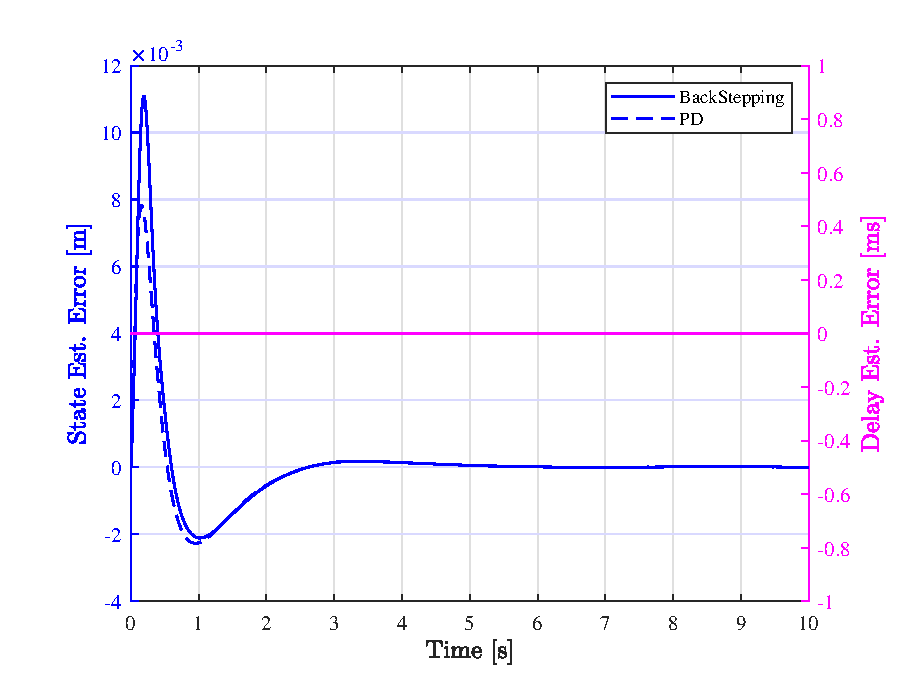
\includegraphics{Figures/RMSEPerfect.eps}}
	\caption{State estimation error with perfect delay estimator}
	\label{fig:Error(PerfectEstLow)}
\end{figure}

Fig.~\ref{fig:U(PerfectEstLow)} shows the control signals calculated on the  Ground Control Station according to the estimated quadrotor states. The control signal for both controllers are similar, and as it is shown in Fig.~\ref{fig:Error(PerfectEstLow)}, the control framework that works based on the PD controller estimates the states similar to the state estimator that works based on the backstepping.

\begin{figure}[H]
	\centerline{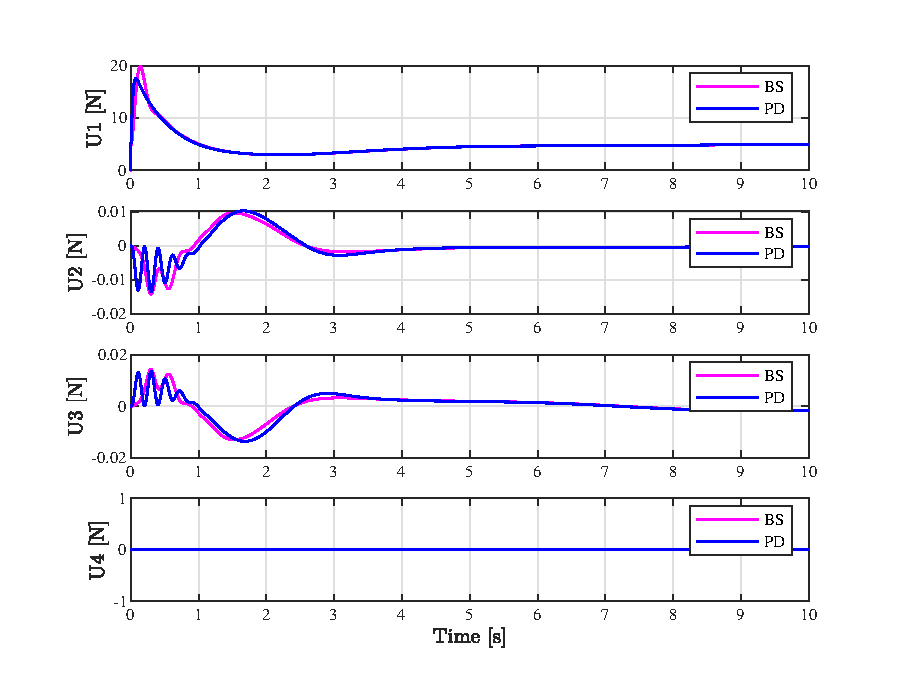
\includegraphics{Figures/UPerfect.eps}}
	\caption{Control signals with perfect delay estimator}
	\label{fig:U(PerfectEstLow)}
\end{figure}

\paragraph{Delay estimation based on the Markov model} In this case, delays were changed based on the predefined transition matrix. According to Fig.~\ref{fig:Error(NormalLow)}, the estimation error for the PD and backstepping controllers did not change significantly due to small delay values. The true and estimated transition probability matrices are shown in Table \ref{Table3.3}.

\begin{table}[H]
	\begin{center}
	\caption{True and estimated transition probabilities}
		\begin{tabular}{|clllll|}
		\hline
		\multicolumn{1}{|l}{}                     &                               & \multicolumn{1}{c}{6 $ms$} & \multicolumn{1}{c}{7 $ms$} & \multicolumn{1}{c}{9 $ms$} & \multicolumn{1}{c|}{10 $ms$} \\ \hline
		\multicolumn{1}{|c|}{\multirow{2}{*}{6 $ms$}}  & \multicolumn{1}{l|}{True}     & 0.7736                & 0.0250                & 0.1643                & 0.0372                  \\
		\multicolumn{1}{|c|}{}                    & \multicolumn{1}{l|}{Estimate} & 0.7631                & 0.0259                & 0.1705                & 0.0405                  \\ \hline
		\multicolumn{1}{|c|}{\multirow{2}{*}{7 $ms$}}  & \multicolumn{1}{l|}{True}     & 0.0224                & 0.1972                & 0.0723                & 0.7080                  \\
		\multicolumn{1}{|c|}{}                    & \multicolumn{1}{l|}{Estimate} & 0.0349                & 0.2170                & 0.0574                & 0.6908                  \\ \hline
		\multicolumn{1}{|c|}{\multirow{2}{*}{9 $ms$}}  & \multicolumn{1}{l|}{True}     & 0.0360                & 0.1797                & 0.0310                & 0.7533                  \\
		\multicolumn{1}{|c|}{}                    & \multicolumn{1}{l|}{Estimate} & 0.0333                & 0.1849                & 0.0258                & 0.7559                  \\ \hline
		\multicolumn{1}{|c|}{\multirow{2}{*}{10 $ms$}} & \multicolumn{1}{l|}{True}     & 0.2097                & 0.0075                & 0.0305                & 0.7523                  \\
		\multicolumn{1}{|c|}{}                    & \multicolumn{1}{l|}{Estimate} & 0.2174                & 0.0072                & 0.0357                & 0.7397                  \\ \hline
		\end{tabular}
		\label{Table3.3}
	\end{center}
\end{table}


\begin{figure}[H]
	\centering
	\centerline{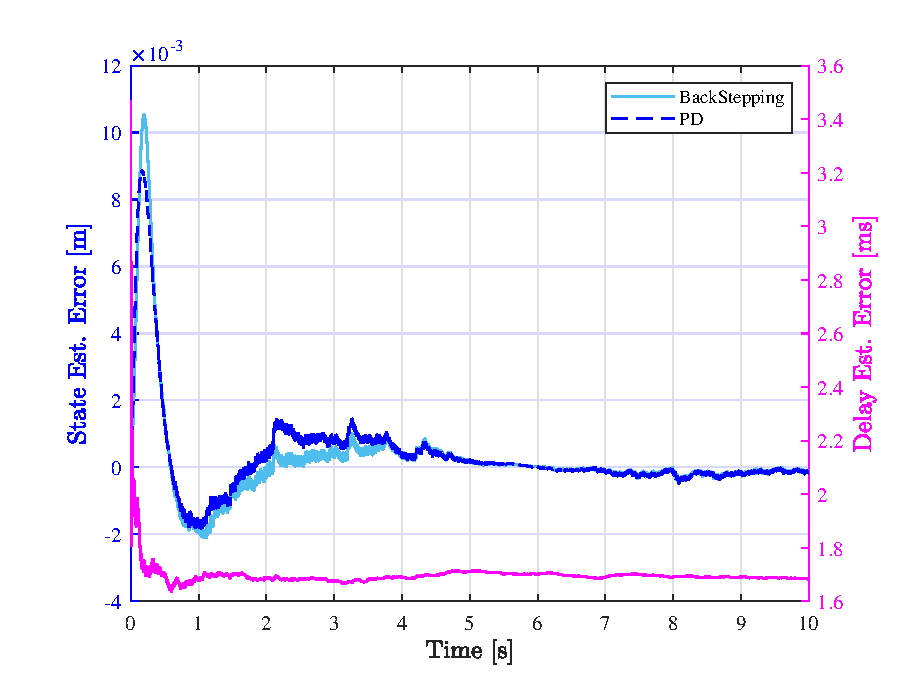
\includegraphics{Figures/RMSENormalLow.eps}}
	\caption{State and delay estimation error for $D=\left\lbrace 6, 7, 9, 10\right\rbrace$ $ms$}
	\label{fig:Error(NormalLow)}
\end{figure}

As illustrated in Fig.~\ref{fig:U(NormalLow)}, even very small unknown delays affect controller performance. Because of the time delay in the system, tiny oscillations happen in the quadrotor's orientation. For example, since the bandwidth of the PD controller is relatively high (large gains in the control signal), small feedback errors are multiplied by the large gains and generate oscillating control signals.

\begin{figure}[H]
	\centerline{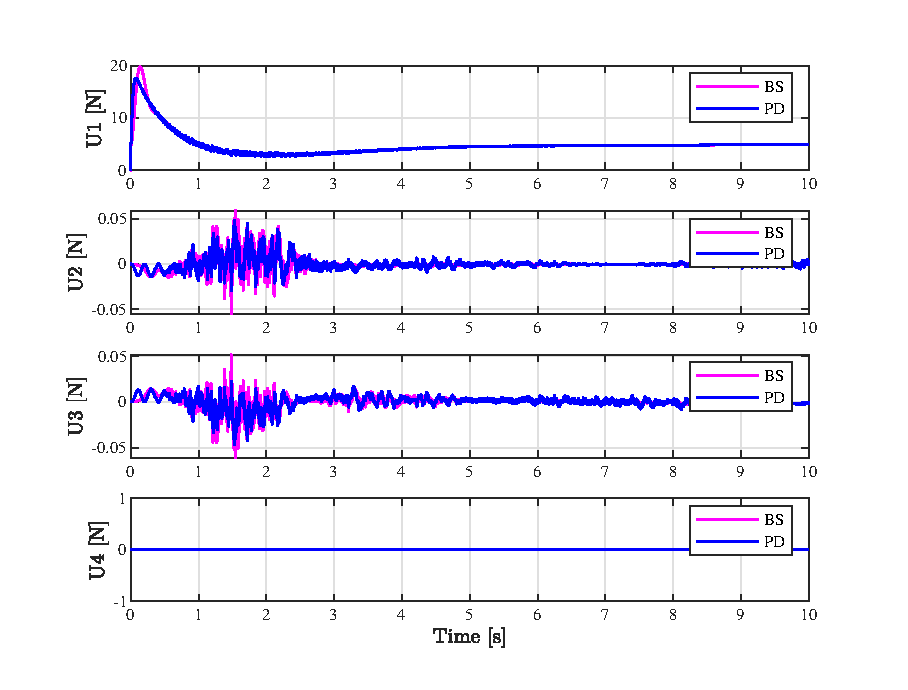
\includegraphics{Figures/UNormalLow.eps}}
	\caption{Control signals for $D=\left\lbrace 6, 7, 9, 10\right\rbrace$ $ms$}
	\label{fig:U(NormalLow)}
\end{figure}

In order to study the effect of the large changes in delay on the system, the time delays were changed to $D=\left\lbrace 1, 3, 13, 15\right\rbrace$ $ms$. The simulation was done with the true transition probabilities presented in Table \ref{Table3.3}. Fig.~\ref{fig:Error(NormalHigh)} shows how a slight change in the delay variation increases the estimation error. It also shows that we cannot use the mean value for the delay because large variations in delay negatively affect the response. It takes longer for the state estimator to estimate the current position.

\begin{figure}[H]
	\centering
	\centerline{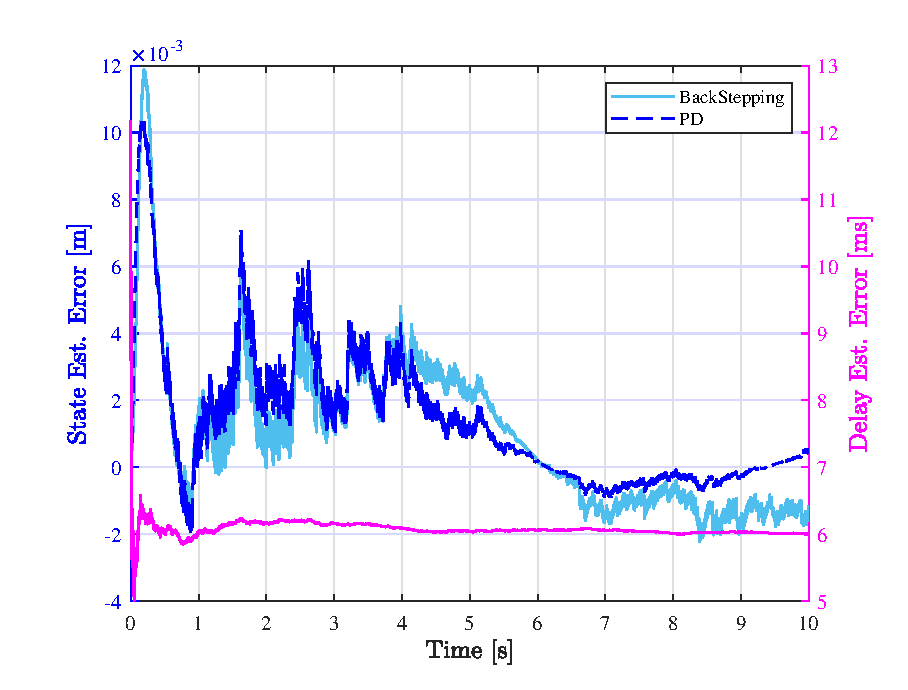
\includegraphics{Figures/RMSENormalHigh.eps}}
	\caption{State and delay estimation error for $D=\left\lbrace 1, 3, 13, 15\right\rbrace$ $ms$}
	\label{fig:Error(NormalHigh)}
\end{figure}

According to Fig.~\ref{fig:U(NormalHigh)}, large variations in state estimation error affect the backstepping controller so that it generates control signals with higher frequency and amplitude than the PD controller. It should be noted that although one way to solve this problem is to reduce the backstepping controller's coefficients, lower values for coefficients increase the response time and path RMSE.

\begin{figure}[H]
	\centerline{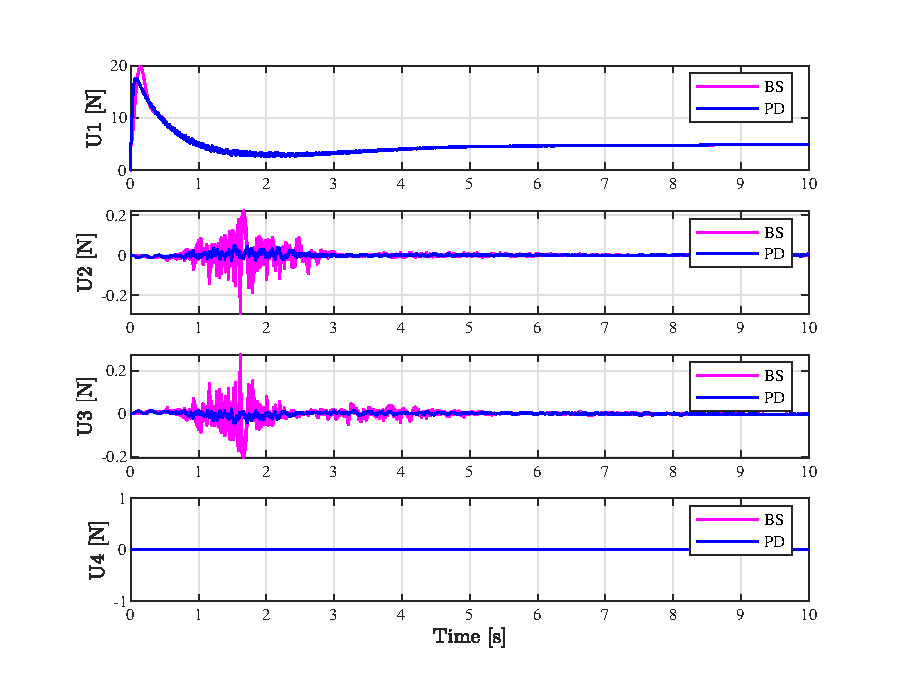
\includegraphics{Figures/UNormalHigh.eps}}
	\caption{Control signals for $D=\left\lbrace 1, 3, 13, 15\right\rbrace$ $ms$}
	\label{fig:U(NormalHigh)}
\end{figure}


\paragraph{Change in delay values and distributions} While the cellular networks provide higher communication bandwidth with lower time delays, the variation in network load in crowded areas like urban environments changes the network properties. During the simulation, the time delays ($D$) and their distributions $p$ were changed to simulate the changes in network states. The simulation was done with delays between $1-10$ $ms$, and the time delay values and their transition probabilities were changed six times.

\begin{figure}[H]
	\centerline{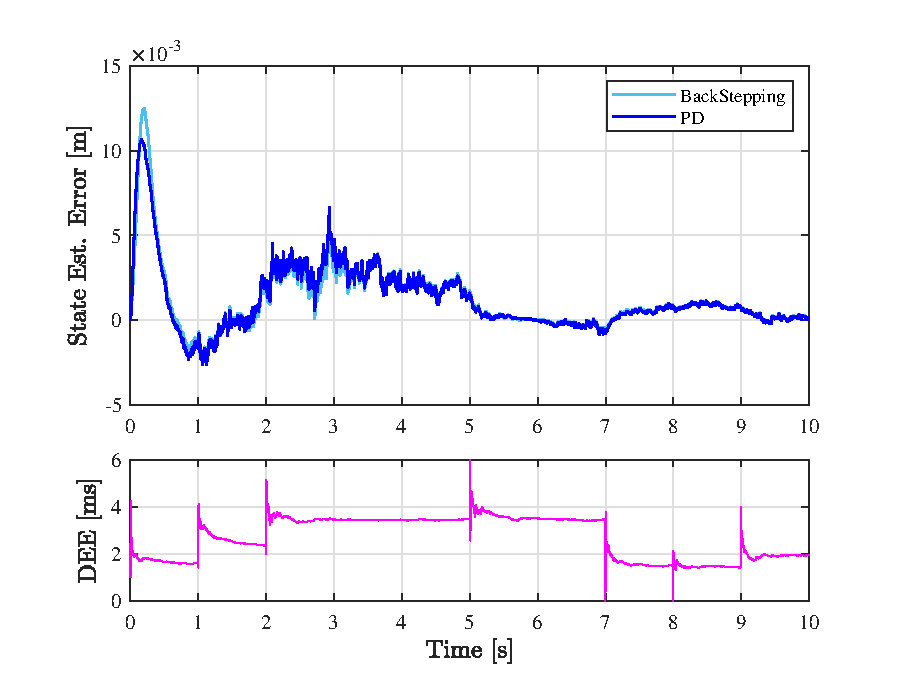
\includegraphics{Figures/RMSEDlyChng.eps}}
	\caption{State and delay estimation error when delays and their distribution changed (Large variations in delay estimation shows the points where the delay values and the transition probabilities are changed)}
	\label{fig:Error(DelayChng)}
\end{figure}

Fig.~\ref{fig:Error(DelayChng)} shows the delay estimation error during the simulation. According to the figure, change in delay values and distributions has affected the delay estimation. However, small delay changes between 1 to 10 $ms$ did not decrease the state estimator's performance. It should be noted that after every change in delay, the DEE was reset, and error was calculated for new time delays.

\begin{figure}[H]
	\centerline{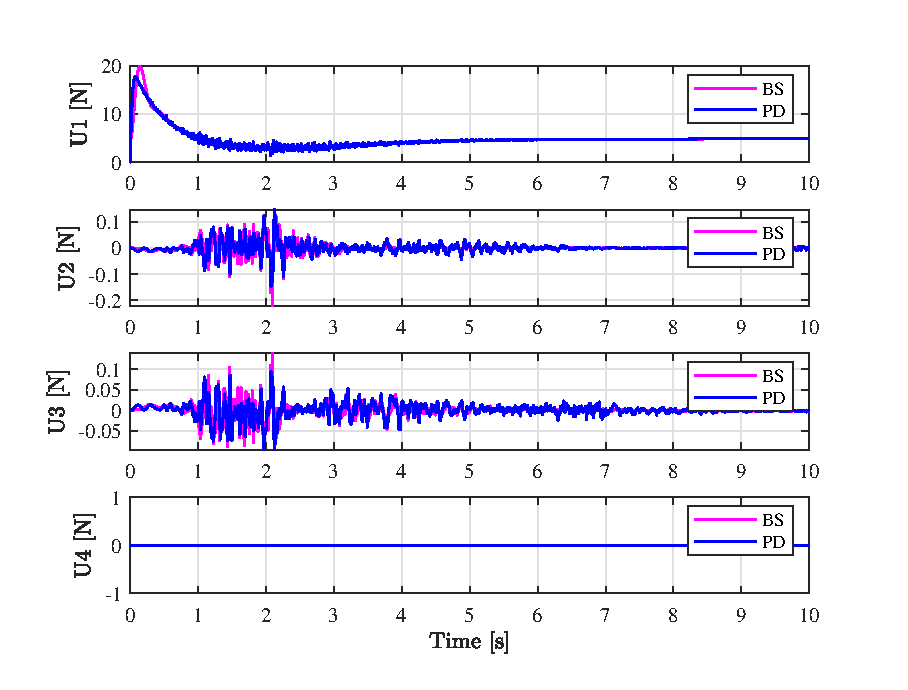
\includegraphics{Figures/UDelayChange.eps}}
	\caption{Control signals when delays and delay distributions changed}
	\label{fig:U(DelayChng)}
\end{figure}

As shown in Fig.~\ref{fig:U(DelayChng)}, errors in estimating time delay caused high-frequency oscillations in the control signal. Although the maximum delay value is not changed, changing delay values between 1 to 10 $ms$ negatively affected the control signal.

According to the results, PD and backstepping controllers have similar performance in quadrotor control. However, in the case of the large variation in time delay, the PD controller generates better control signals. The design process of the backstepping controller is more complicated than the PD controller.

In this chapter, the PD gains and backstepping coefficients were set so that the trajectory tracking performance was almost the same. RMSE of the path in $x$, $y$, and $z$ directions were 1.046, 1.138, and 0.131 $m$ for the PD controller, and 1.224, 1.329, and 0.19 $m$ for the backstepping controller. In this case, the forward delay is the major reason for high RMSE and makes quadrotor follow the path with delay. 

In the linear PD controller, the gains can be tuned using inner and outer loop bandwidths. Also, using the theoretical stability analysis based on the linearized model, one can find an equation between time delay and controller's bandwidth. This issue helps the control framework adjust the bandwidth based on the observed time delay. 

The bandwidth adaptation in the backstepping controller is a complex task since 12 parameters should be tuned. On the other hand, developing an equation between coefficients and time delay is much more complex than the linear PD controller.

Cellular networks are state-of-the-art communication tools for precise swarm control of drones. The presented control framework can control multiple drones from the GCS while the state estimator provides precise information about each drone's current position and orientation (fully observable system) for real-time centralized multi-agent-based collision avoidance, cooperation, and path planning tasks.

\section{Experimental setup}

